\section{Расчет коэффициента обратной связи, сравнение с результатами Дваера}\label{sec:thunderstorm/rdfm}
% Gurevich2000.pdf --- даны оценки числа рожденных электрон-позитронных пар
Несмотря на то что в хороших условиях в лавине убегающих электронов может быть сгенерировано более миллиона дополнительных электронов (см.~\ref{sec:thunderstorm/rrea}), это не объясняет большие потоки гамма-квантов в TGF, а также не дает объяснения как связанны между собой процессы с высокоэнергетичными частицами и разряды молнии. Одним из вариантов модификации теории Гуревича, является построение на её основе модели с обратной связью (ОС). Джозеф Дуайер в работе~\cite{dwyer2003fundamental} предложил рассмотреть два механизма которые могут привести к возникновению обратной связи: гамма обратная связь возникает за счет того что не смотря на то что рождаемые убегающими электронами гамма-квант имеют начальный импульс сонаправленный с направление движения лавины, часть из них в результате рассеяния может в итоге оказаться в части облака в котором начиналась лавина и выбить там электрон, который станет новым затравочным электроном, позитронная обратная связь возникает за счет конверсии гамма-квантов электрон-позитронные пары, при этом позитрон имеет шанс развернутся в электрическом поле и начать ускорятся против направления распространения лавины, выбивая вторичные электроны, которые опять же имеют шанс развернутся в электрическом поле и стать новым затравочным электроном. Рисунок проведенного мною моделирования, иллюстрирует описание позитронной обратной связи: красные треки отображают лавину убегающих электронов, зеленные треки тормозные гамма-кванты, синий трек показывает позитрон обратной связи, который как мы видим создает новые затравочные электроны (которые правда не создают новую лавину). Механизмы описанные Дуайером должны работать в широком диапазоне атмосферных условий, однако являются вероятностными и возникает вопрос насколько значителен вклад этих механизмов в развитие лавин убегающих электронов. В работе~\cite{skeltved2014} повторялись результаты Дуайера, однако без углубленного анализа. В данной работе мы попробуем глубже рассмотреть работу этих механизмов.

\begin{figure}[ph!]
    \begin{center}
        \includegraphics[width=0.8\linewidth]{thunderstorm/ayss_2018_art/10_dwyer.pdf}
        \caption{Распространение лавины убегающих электронов, красные треки --- электроны, зеленые треки --- гамма-кванты, синий трек --- позитрон.}
    \end{center}
    \label{fig:storm:dwyer}
\end{figure}

В работе~\cite{dwyer2003fundamental} приводятся результаты моделирования при нормальных условиях исследующие при каких соотношениях длины области с электрическим полем и величины поля может возникать обратная связь. Синяя линия на графике~\ref{fig:storm:dwyer2003} отображает результат полученный Дуайером в ~\cite{dwyer2003fundamental} при значения электрического поля и длины выше этой кривой возникает положительная обратная связь, которая ведёт к значительному росту новых затравочных частиц, который приводит в возникновению TGF и активной ионизации облака достаточной для разряда молнии, в частности подобный результат также говорит что внутри облаков не должно быть скрытых областей с сильным полем --- подобные области должны быстро разряжаться в следствии действия механизмов обратной связи.

Для проверки данных результатов было проведено собственное моделирование, состоящее из двух частей:
\begin{itemize}
	\item Моделирование рождения новых затравочных электронов (аналогично работе~\cite{dwyer2003fundamental} электрон считался новым затравочным, если рождался в от гамма-кванта или позитрона в верхней половине облака)за счет гамма и позитронной обратной связи за одну итерацию на одну первичную частицу.
	\item Расчет вероятности с которой электрон может развернутся в электрическом поле. 
\end{itemize}
Для оценки вероятности разворота было проведено GEANT4 моделирование, для сухого воздуха при нормальных условиях, величины электрического поля бралась от 5 до 10 кВ/см с шагом 0.5 кВ/см. Результат расчета вероятности разворота представлена на рисунках~\ref{fig:storm:reverse_nc_1} и ~\ref{fig:storm:reverse_nc_2}. Так же что бы быть уверенным что электрон после разворота сможет начать движение была рассчитана средняя энергия электрона после разворота, результаты приведены на графиках~\ref{fig:storm:reverse_energy_nc_1} и ~\ref{fig:storm:reverse_energy_nc_2}, как видно из графиков хоть электрон и тратит энергию на разворот, она остается достаточной для запуска новой лавины убегающих электронов (см. график ~\ref{fig:storm:gurevich}б), показывающий минимальную энергию для начала убегания).  

\begin{figure}[ph!]
    \begin{center}
        \begin{minipage}[h]{0.49\linewidth}
            \center{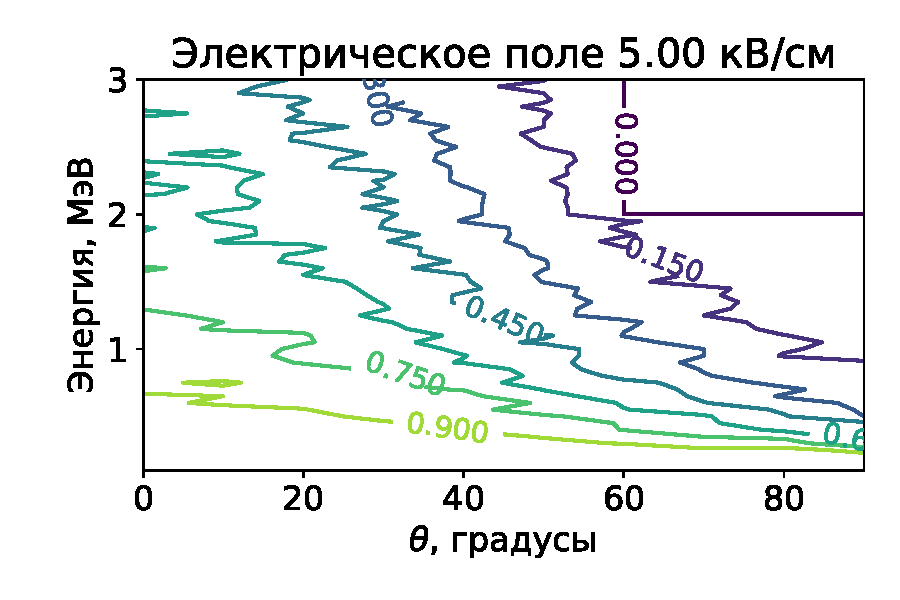
\includegraphics[width=\linewidth]{thunderstorm/rdfm/reverse_5_00.pdf} \\ а)}
        \end{minipage}
        \hfill
        \begin{minipage}[h]{0.49\linewidth}
            \center{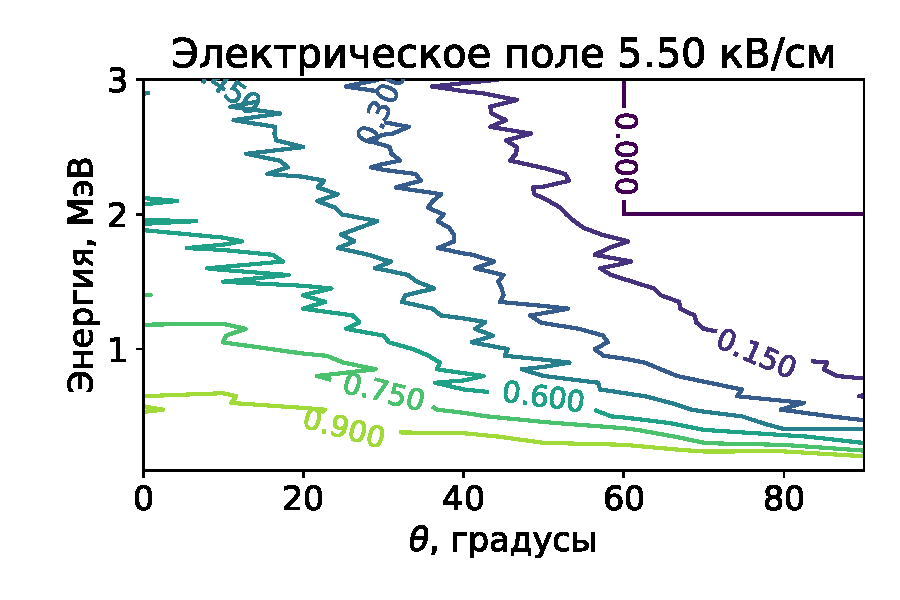
\includegraphics[width=\linewidth]{thunderstorm/rdfm/reverse_5_50.pdf} \\ б)}
        \end{minipage}
        \vfill
        \begin{minipage}[h]{0.49\linewidth}
            \center{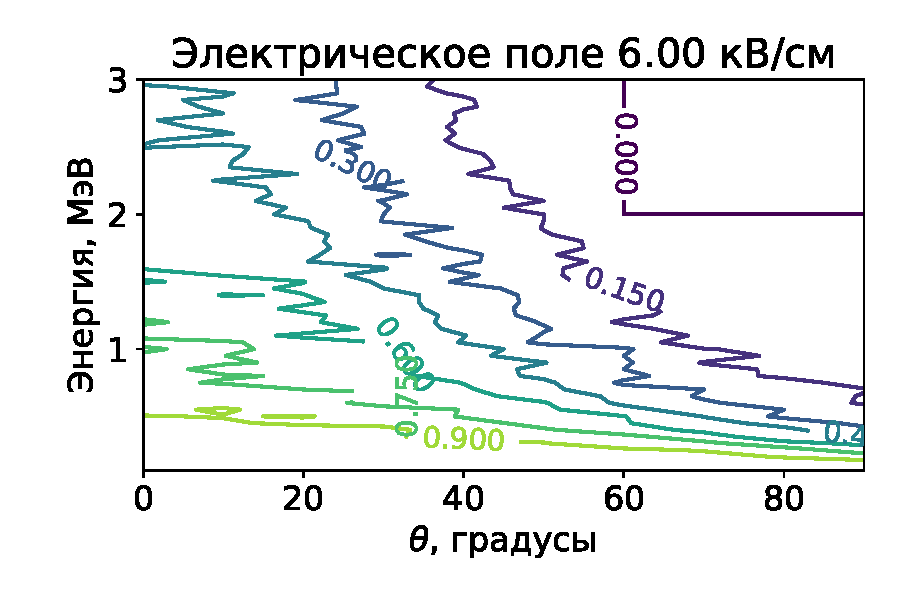
\includegraphics[width=\linewidth]{thunderstorm/rdfm/reverse_6_00.pdf} \\ в)}
        \end{minipage}
        \hfill
        \begin{minipage}[h]{0.49\linewidth}
            \center{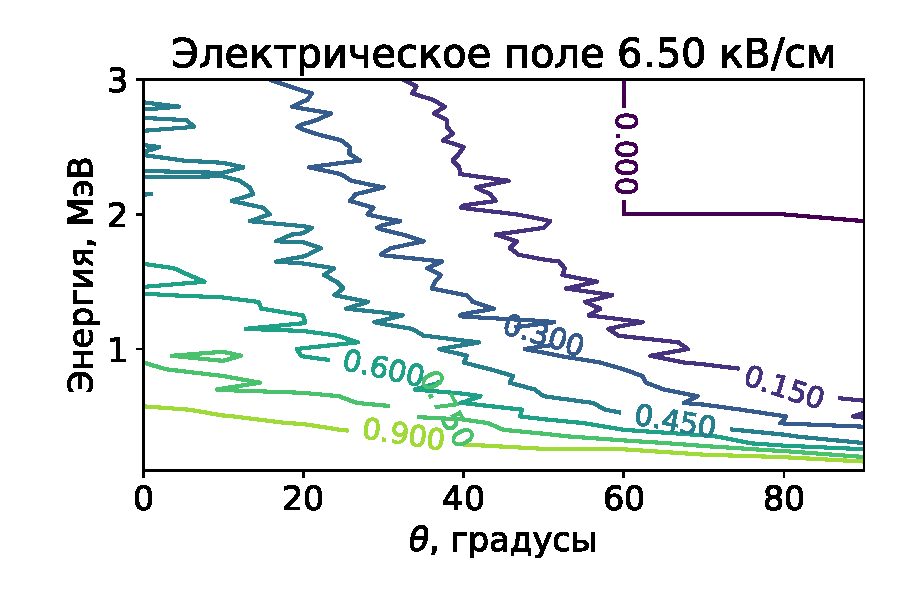
\includegraphics[width=\linewidth]{thunderstorm/rdfm/reverse_6_50.pdf} \\ г)}
        \end{minipage}
        \vfill
        \begin{minipage}[h]{0.49\linewidth}
            \center{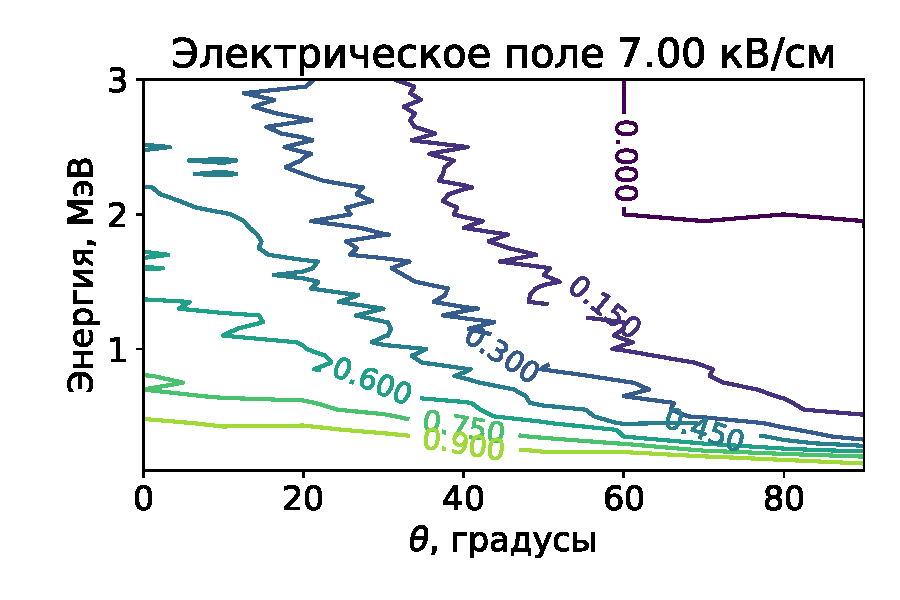
\includegraphics[width=\linewidth]{thunderstorm/rdfm/reverse_7_00.pdf} \\ д)}
        \end{minipage}
        \hfill
        \begin{minipage}[h]{0.49\linewidth}
            \center{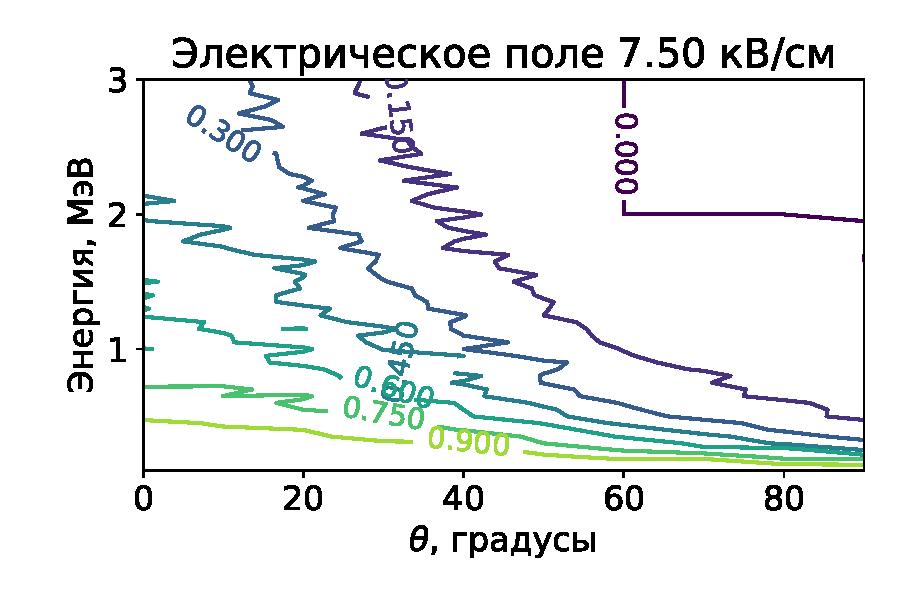
\includegraphics[width=\linewidth]{thunderstorm/rdfm/reverse_7_50.pdf} \\ е)}
        \end{minipage}
        \caption{Расчет вероятности электрона развернутся в электрическом поле для нормальных условий. По оси X отображается угол между направление движения TODO(перерисовать угол на графике), а по оси Y энергия электронов. На графики отображены линии с постоянной вероятность разворота и числовое значение вероятности на линии.}
    \end{center}
    \label{fig:storm:reverse_nc_1}
\end{figure}
\begin{figure}[ph!]
    \begin{center}
        \begin{minipage}[h]{0.49\linewidth}
            \center{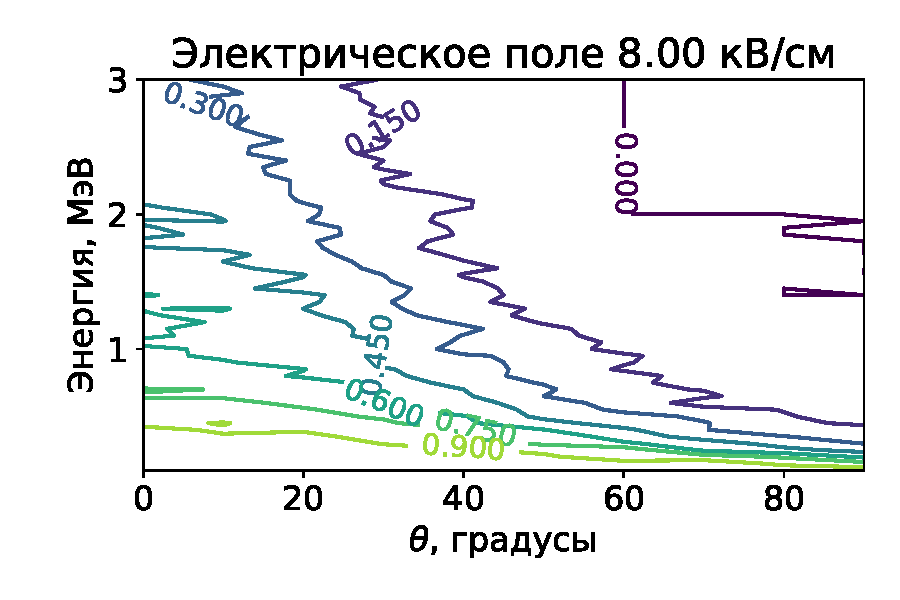
\includegraphics[width=\linewidth]{thunderstorm/rdfm/reverse_8_00.pdf} \\ ж)}
        \end{minipage}
        \hfill
        \begin{minipage}[h]{0.49\linewidth}
            \center{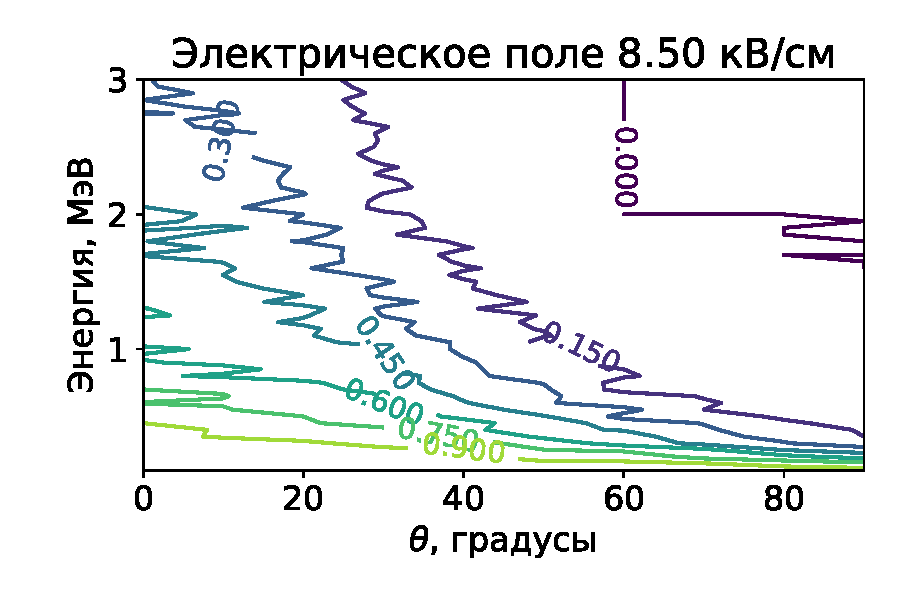
\includegraphics[width=\linewidth]{thunderstorm/rdfm/reverse_8_50.pdf} \\ з)}
        \end{minipage}    
        \vfill
        \begin{minipage}[h]{0.49\linewidth}
            \center{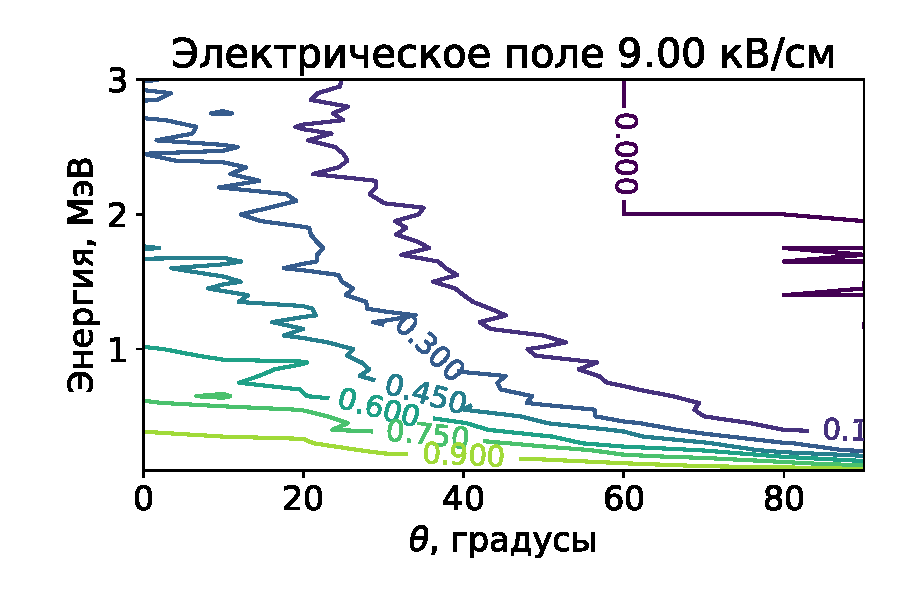
\includegraphics[width=\linewidth]{thunderstorm/rdfm/reverse_9_00.pdf} \\ и)}
        \end{minipage}
        \hfill
        \begin{minipage}[h]{0.49\linewidth}
            \center{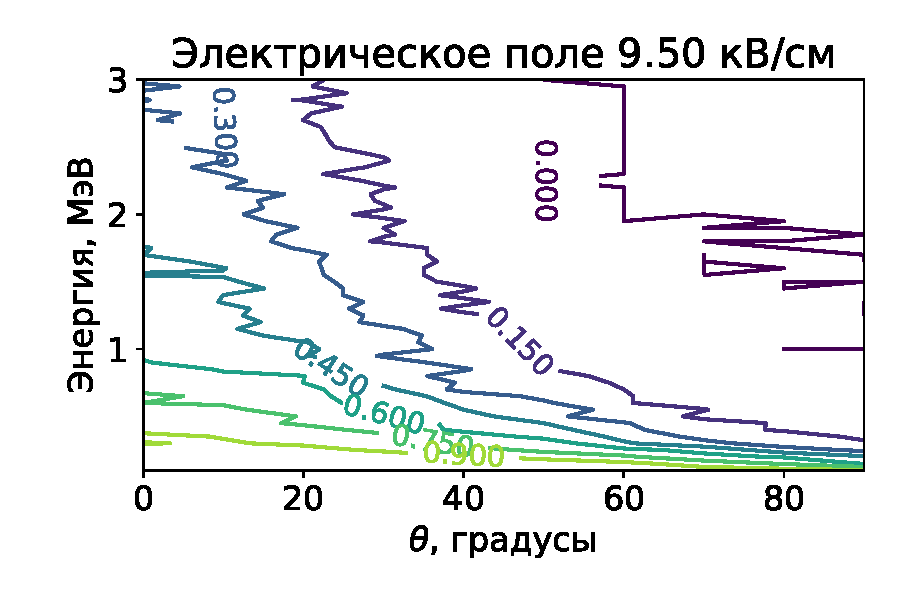
\includegraphics[width=\linewidth]{thunderstorm/rdfm/reverse_9_50.pdf} \\ к)}
        \end{minipage} 
        \vfill
        \begin{minipage}[h]{0.49\linewidth}
            \center{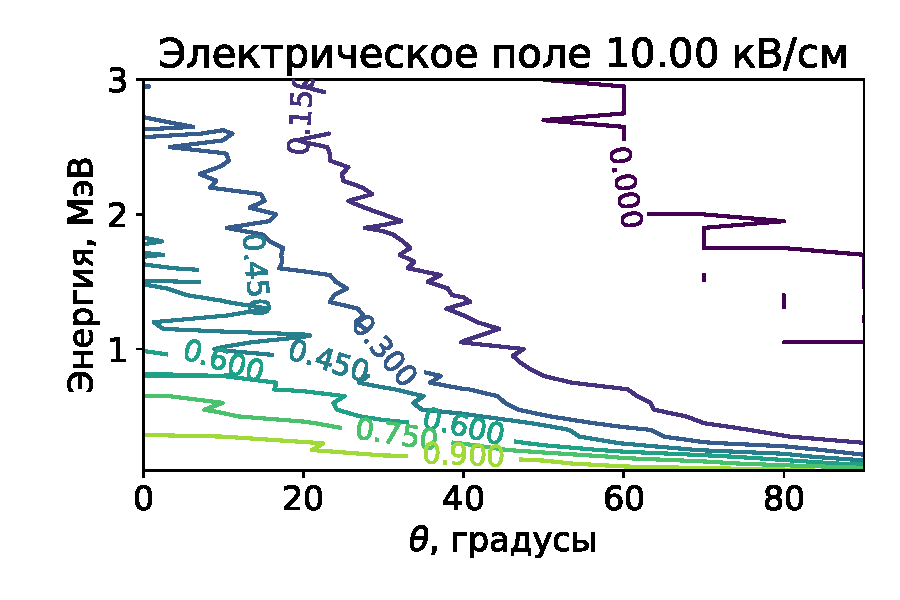
\includegraphics[width=\linewidth]{thunderstorm/rdfm/reverse_10_00.pdf} \\ л)}
        \end{minipage}
        \caption{Разворот электрона TODO(Скопировать)}
    \end{center}
    \label{fig:storm:reverse_nc_2}
\end{figure}


\begin{figure}[ph!]
    \begin{center}
        \begin{minipage}[h]{0.49\linewidth}
            \center{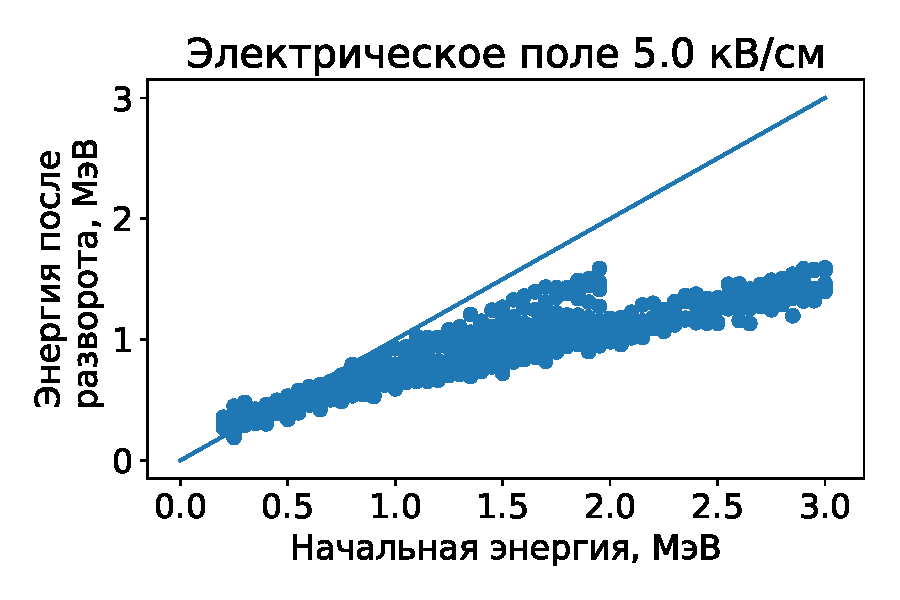
\includegraphics[width=\linewidth]{thunderstorm/rdfm/reverse_energy_5_0.pdf} \\ а)}
        \end{minipage}
        \hfill
        \begin{minipage}[h]{0.49\linewidth}
            \center{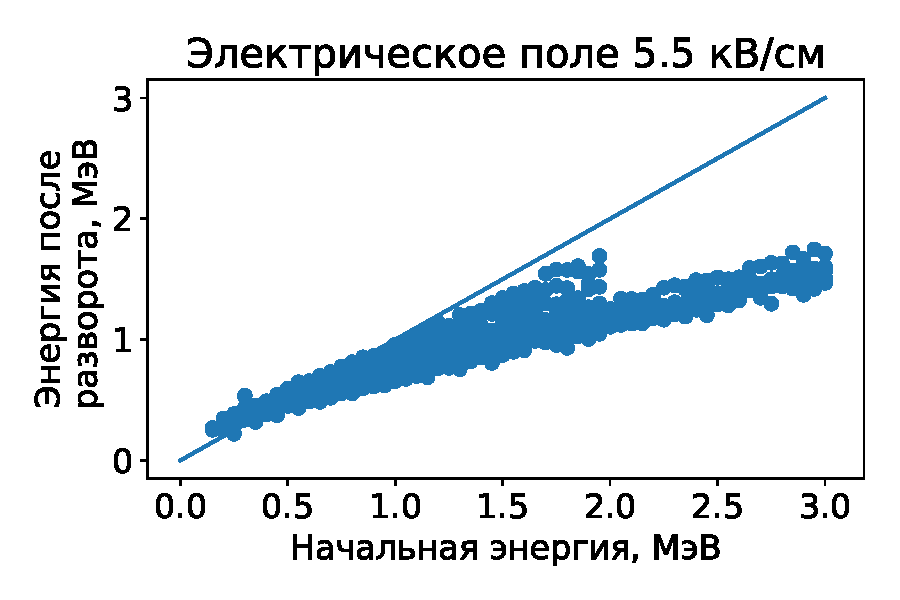
\includegraphics[width=\linewidth]{thunderstorm/rdfm/reverse_energy_5_5.pdf} \\ б)}
        \end{minipage}
        \vfill
        \begin{minipage}[h]{0.49\linewidth}
            \center{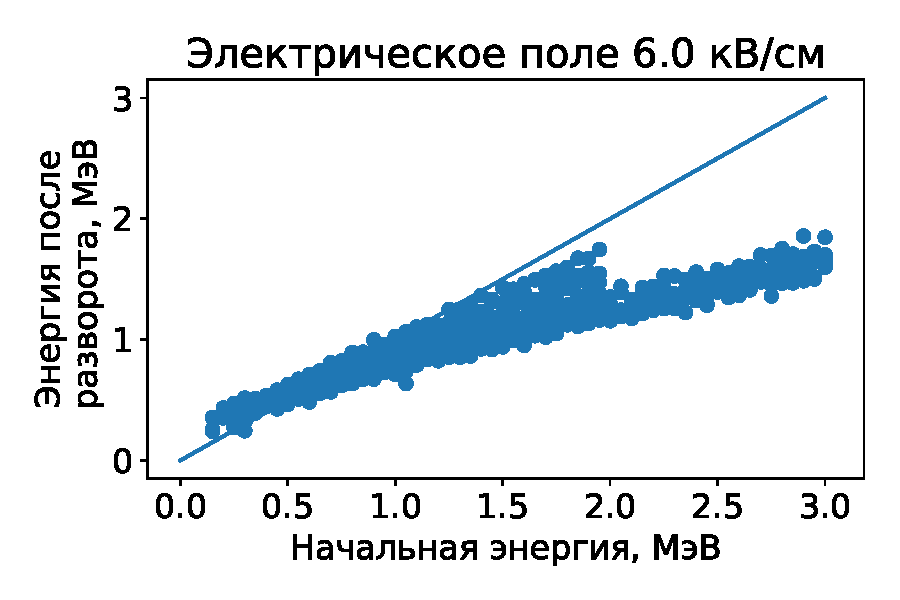
\includegraphics[width=\linewidth]{thunderstorm/rdfm/reverse_energy_6_0.pdf} \\ в)}
        \end{minipage}
        \hfill
        \begin{minipage}[h]{0.49\linewidth}
            \center{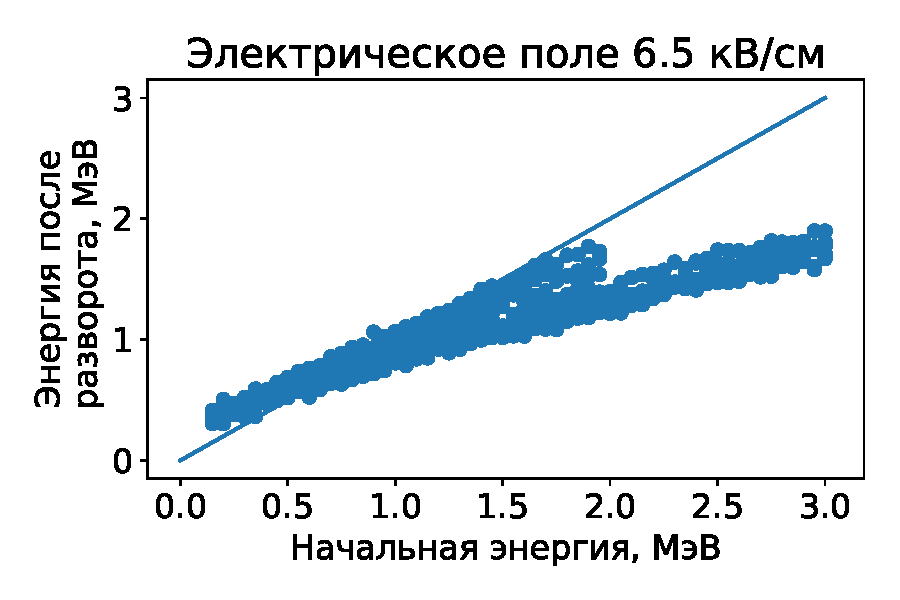
\includegraphics[width=\linewidth]{thunderstorm/rdfm/reverse_energy_6_5.pdf} \\ г)}
        \end{minipage}
        \vfill
        \begin{minipage}[h]{0.49\linewidth}
            \center{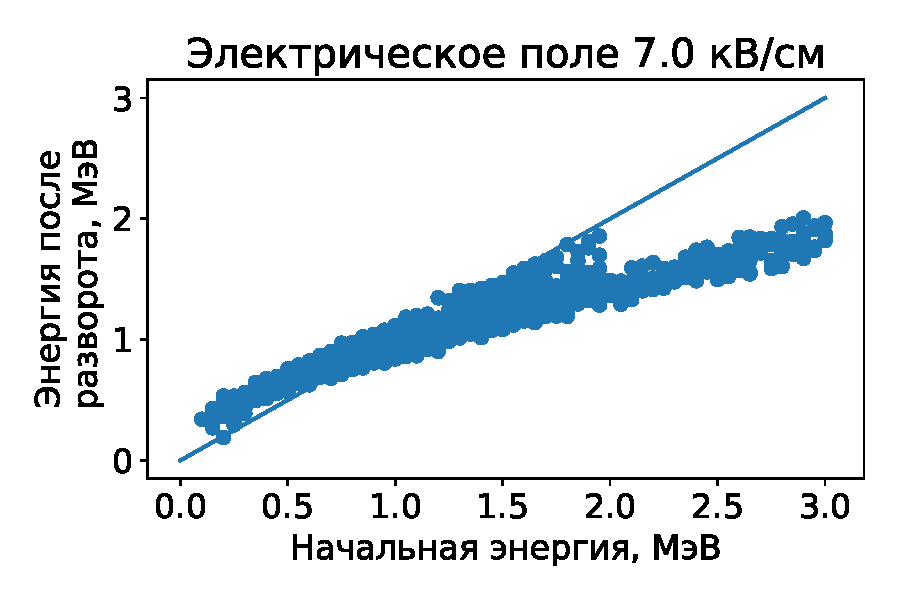
\includegraphics[width=\linewidth]{thunderstorm/rdfm/reverse_energy_7_0.pdf} \\ д)}
        \end{minipage}
        \hfill
        \begin{minipage}[h]{0.49\linewidth}
            \center{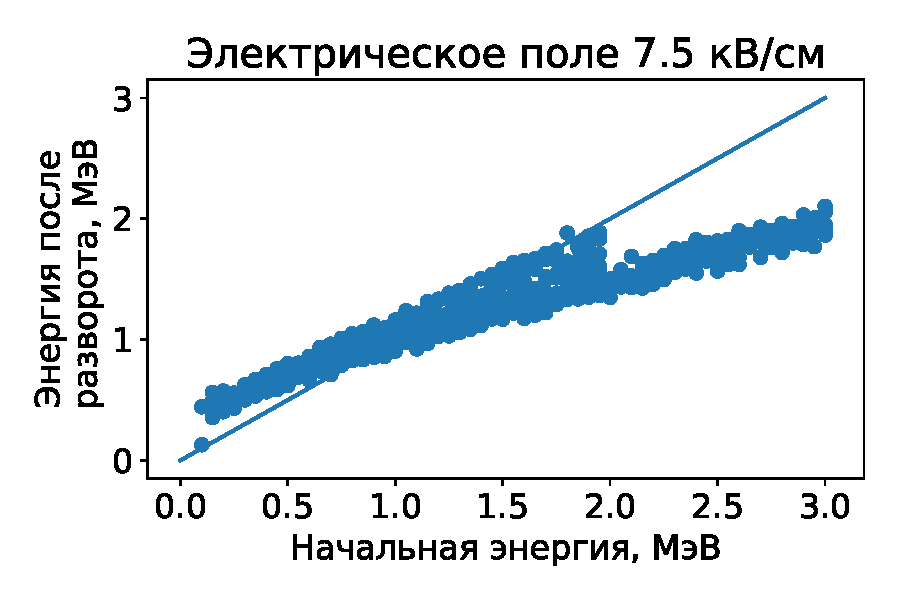
\includegraphics[width=\linewidth]{thunderstorm/rdfm/reverse_energy_7_5.pdf} \\ е)}
        \end{minipage}
        \caption{Зависимость средней энергии электрона после разворота от начальной энергии для разных значений электрического поля.}
    \end{center}
    \label{fig:storm:reverse_energy_nc_1}
\end{figure}
\begin{figure}[ph!]
    \begin{center}
        \begin{minipage}[h]{0.49\linewidth}
            \center{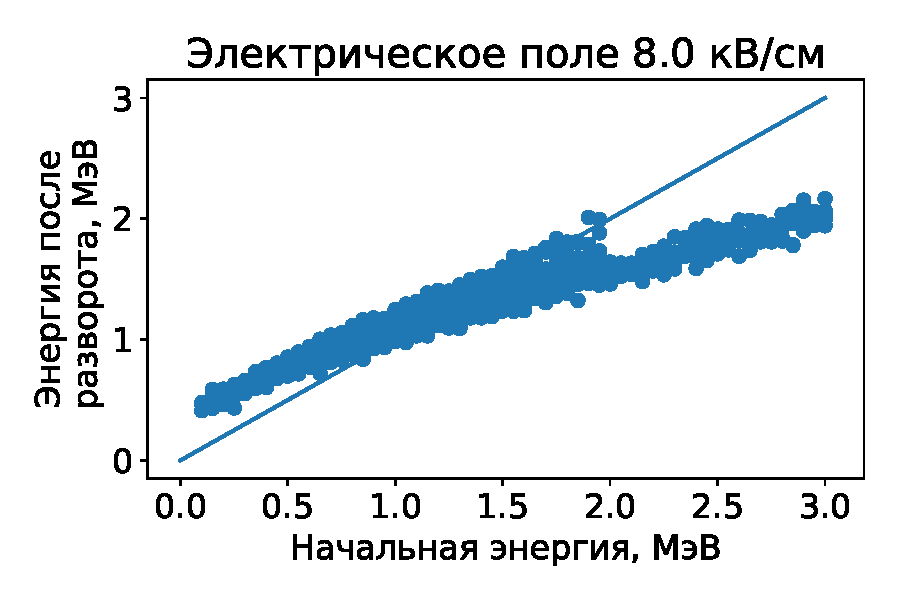
\includegraphics[width=\linewidth]{thunderstorm/rdfm/reverse_energy_8_0.pdf} \\ ж)}
        \end{minipage}
        \hfill
        \begin{minipage}[h]{0.49\linewidth}
            \center{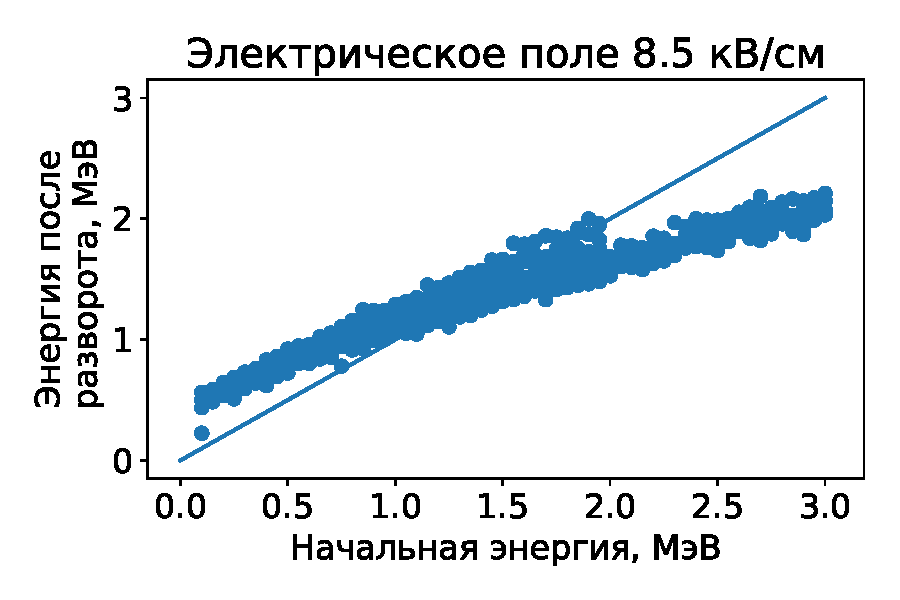
\includegraphics[width=\linewidth]{thunderstorm/rdfm/reverse_energy_8_5.pdf} \\ з)}
        \end{minipage}    
        \vfill
        \begin{minipage}[h]{0.49\linewidth}
            \center{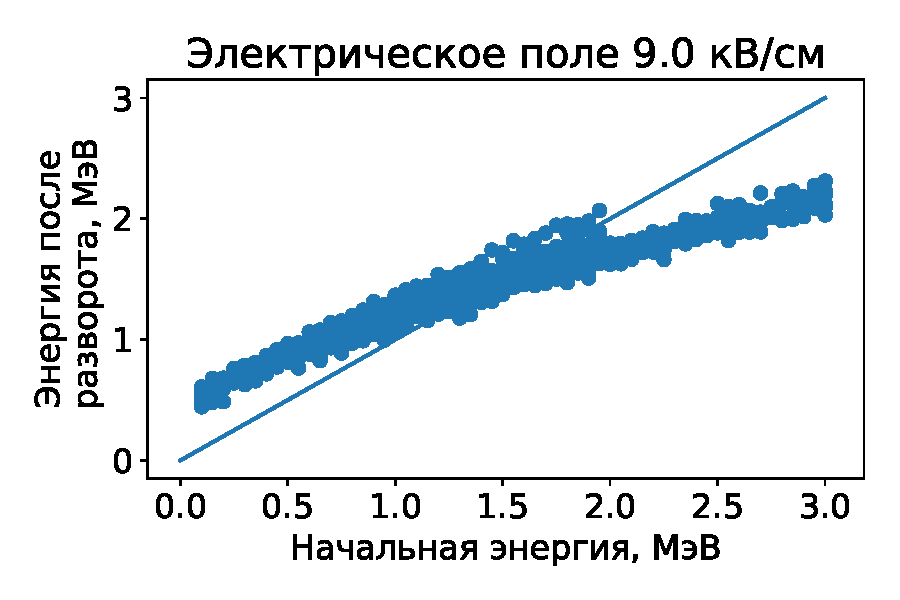
\includegraphics[width=\linewidth]{thunderstorm/rdfm/reverse_energy_9_0.pdf} \\ и)}
        \end{minipage}
        \hfill
        \begin{minipage}[h]{0.49\linewidth}
            \center{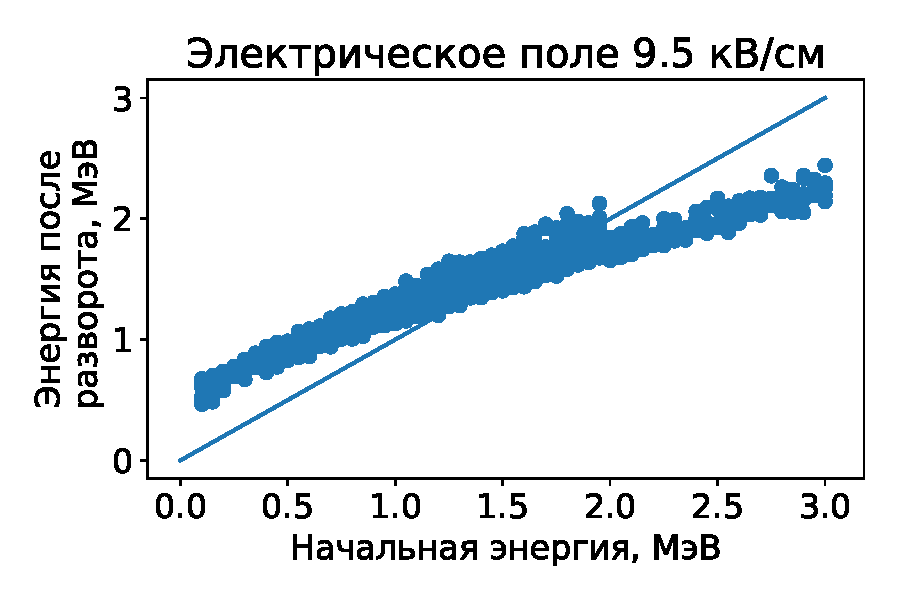
\includegraphics[width=\linewidth]{thunderstorm/rdfm/reverse_energy_9_5.pdf} \\ к)}
        \end{minipage} 
        \vfill
        \begin{minipage}[h]{0.49\linewidth}
            \center{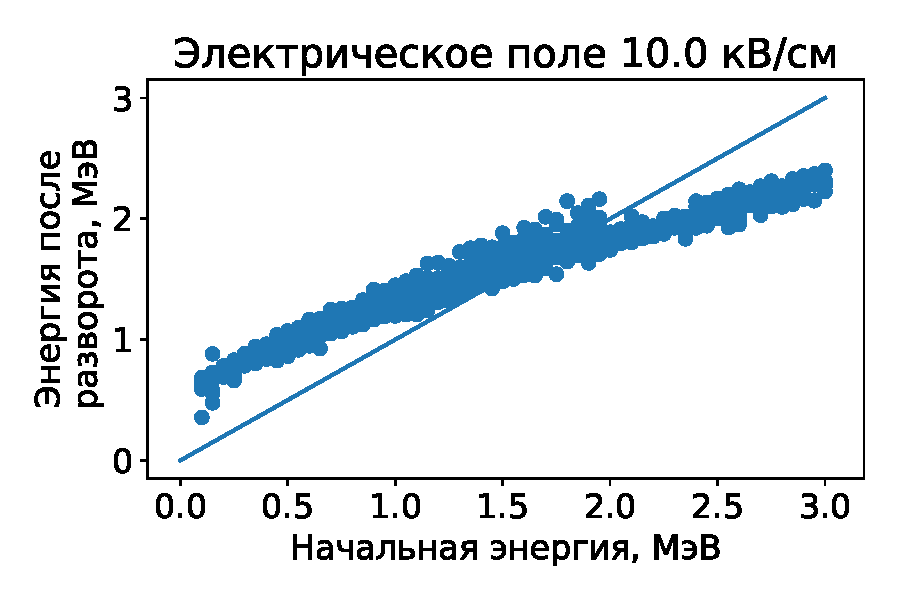
\includegraphics[width=\linewidth]{thunderstorm/rdfm/reverse_energy_10_0.pdf} \\ л)}
        \end{minipage}
        \caption{Зависимость средней энергии электрона после разворота от начальной энергии для разных значений электрического поля.}
    \end{center}
    \label{fig:storm:reverse_energy_nc_2}
\end{figure}
Далее было проведено моделирование рождения новых затравочных электронов, для этого было взято несколько точек вдоль и чуть выше кривой полученной Дуайером (отмечены на графике~\ref{fig:storm:dwyer2003}а красными треугольниками), и для данных точек было сделано GEANT4 моделирование лавины убегающих электронов.  Для каждой точки было рассчитано число новых затравочных электронов рожденных с помощью позитронов и гамма-квантов с учетом вероятности развернутся в электрическом поле, результаты представлены в таблице~\ref{tab:storm:dwyer}. Из проведенного моделирования можно сделать следующие выводы:
\begin{itemize}
	\item Результаты моделирования согласуются с результатами Дуаера, однако в отличии от него мы получили не просто качественную оценку наличия/отсутствия новых затравочных частиц, но и получили количественные оценки, также далее мы проведем структурный анализ новых затравочных электронов и покажем некоторые проблемы которые могут значительно уменьшать эффективность работы механизмов обратной связи.
	\item Наша количественная оценка позволяет сделать интересное наблюдение: на эффективность работы механизмов обратной связи в большей степени влияет длинна области с полем, чем величина поля. Это важный результат так как он говорит о проблемах стримерной гипотезы возникновения TGF, подробнее см раздел TODO(Раздел). 
\end{itemize}

\begin{figure}[t]
    \begin{center}
        \begin{minipage}[h]{0.49\linewidth}
            \center{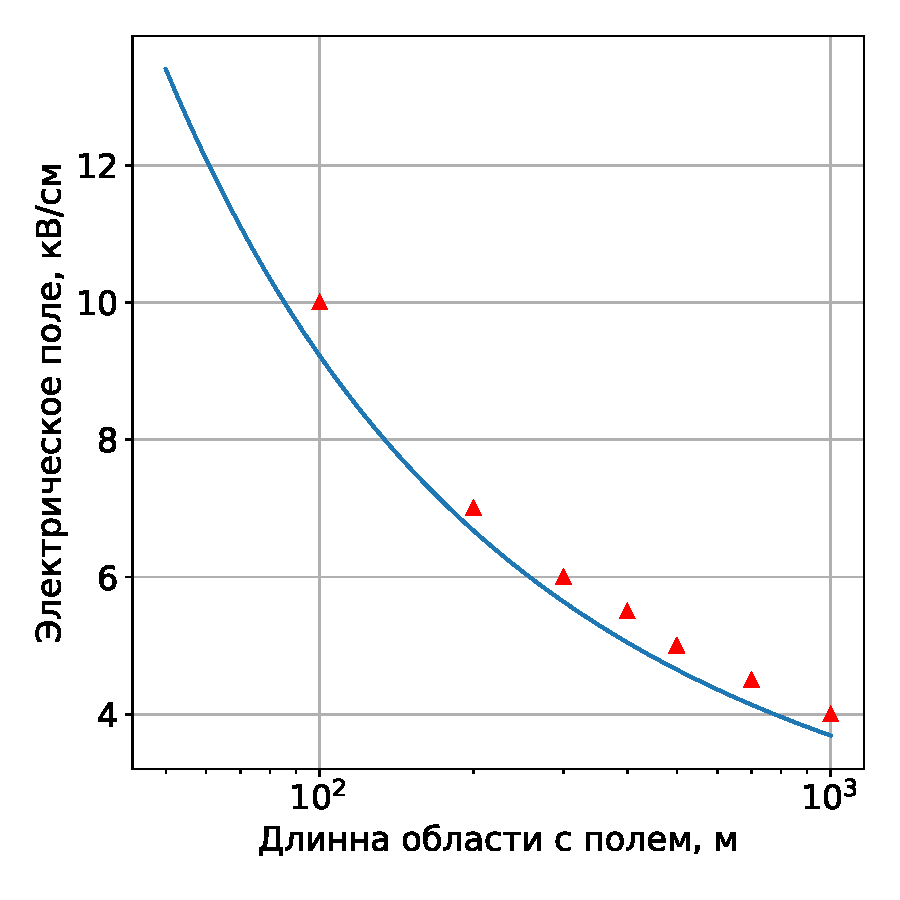
\includegraphics[width=\linewidth]{thunderstorm/rdfm/dwyer_2003.pdf} \\ а)}
        \end{minipage}
        \hfill
        \begin{minipage}[h]{0.49\linewidth}
            \center{\includegraphics[width=\linewidth]{thunderstorm/epl2020/radial-eps-converted-to.pdf}   \\ б)}
        \end{minipage}
        \caption{а) Затухание лавины. б) placeholder.}
    \end{center}
    \label{fig:storm:dwyer2003}
\end{figure}

\begin{table}[h]
    \centering
    \begin{tabular}{crrrr}
        \hline
        & & & \multicolumn{2}{r}{Число новых затравочных электронов} \\
        & Поле, кВ/см &  Длина облака, м  & от гамма ОС & от позитронной ОС \\
        \hline
        & 4   &  1000&  0 & 0  \\
        & 4.5 &  700 &  200 ($\pm 10 \%$)& 400 ($\pm 5 \%$) \\
        & 5   &  500 &  100 ($\pm 14 \%$)& 40 ($\pm 5 \%$) \\
        & 5.5 &  400 &  110 ($\pm 3 \%$)& 85 ($\pm 5 \%$) \\
        & 6   &  300 &  40 ($\pm 3 \%$)& 70 ($\pm 2 \%$) \\
        & 7   &  200 &  7 ($\pm 2 \%$)& 8 ($\pm 2 \%$) \\
        & 10  &  100 &  5 ($\pm 3 \%$)& 2 ($\pm 5 \%$) \\
        \hline
    \end{tabular}
    \caption{Моделирование числа новых затравочных электронов возникающих за счет одной итерации механизма обратной связи на один первичный электрон.}
    \label{tab:storm:dwyer}
\end{table}

Однако не смотря на то что наши результат совпали с результатами Дуайера, у его модели обратной связи можно отметить несколько недостатков. 

Моделирование Дуайера проводилось при нормальных условиях, то есть для атмосферы лежащей на уровне моря, однако реальные явления происходят больших высотах (например, на научных станциях на г. Арагац и на Тянь Шане производится наблюдение за грозовыми облаками идущими на высотах 3-5 километра, а спутниковые наблюдения говорят об источниках TGF расположенных на высотах 12-15 километров). Можно провести экстраполяцию от нормальных условий к условиям на больших высотах, считая что величины (такие как критическое  поле или поле для возникновения обратной связи) уменьшаются пропорционально плотности, а расстояния увеличиваются пропорционально плотности, как было предложен Дуайером, однако такие предположения имеет ограниченную точность. Например, проведенный в разделе ~\ref{sec:thunderstorm/rrea} расчет характерной длинны нарастания лавины был проведен при условиях соответствующей 10 километровой высоте и сравнивался с величиной полученной Дуайером, которая была рассчитана при нормальных условиях и экстраполирована к условия высота 10 км, полученные результат отличаются, хоть они и не дают такого различия как результаты полученные в работе~\cite{oreshkin2018}, но в рамках сравнения наших моделирований отличие существенно и может свидетельствовать он не правомерности интерполяции результатов полученных при нормальных условиях к условиях на больших высотах. 

Другим недостатком расчетов Дуайера является пренебрежение реальными размерами облака, для примера рассмотрим радиальное распределение рождения убегающих электронов показанное на рис.~\ref{fig:storm:dwyer2003}б, которое соответствует облаку на высоте 10 км. Видно, что электроны имеют широкое горизонтальное распределение которое может быть сравнимым с размером небольшого облака. Дополнительно следует учесть что фотоны могут переносить вторичные лавины далеко от начальных, или активно покидать облако. Если построить радиальные распределения рожденных новых затравочных электронов для точек из таблицы~\ref{tab:storm:dwyer}, то можно у видеть что для них также характерен широкий (более 500 метров) разброс, таким образом для облака с характерным размером порядка 1 километра, частицы уже во время второй или третей итерации обратной связи будут покидать облако и перестанут ускорятся. 
\begin{figure}[t]
    \begin{center}
        \begin{minipage}[h]{0.49\linewidth}
            \center{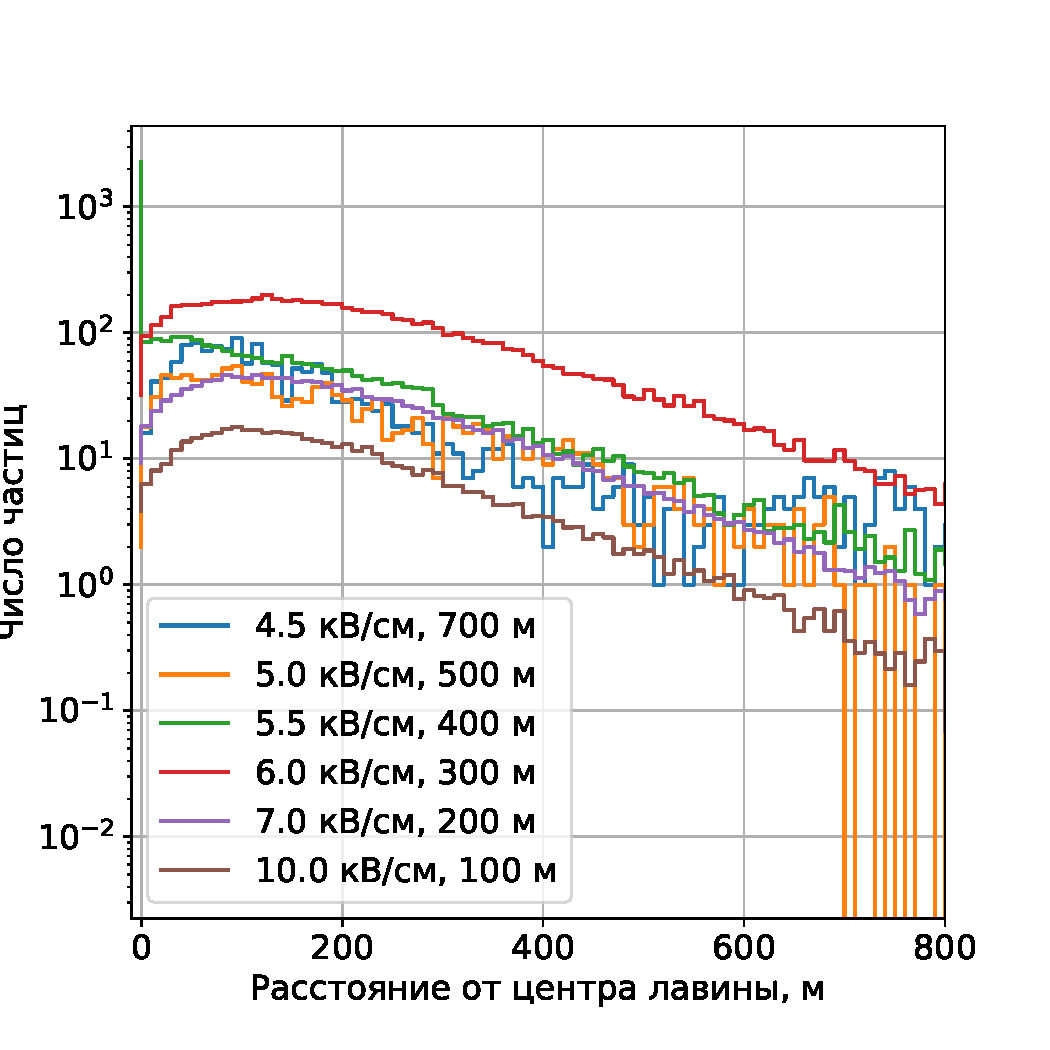
\includegraphics[width=\linewidth]{thunderstorm/rdfm/radial_gamma.pdf} \\ а)}
        \end{minipage}
        \hfill
        \begin{minipage}[h]{0.49\linewidth}
            \center{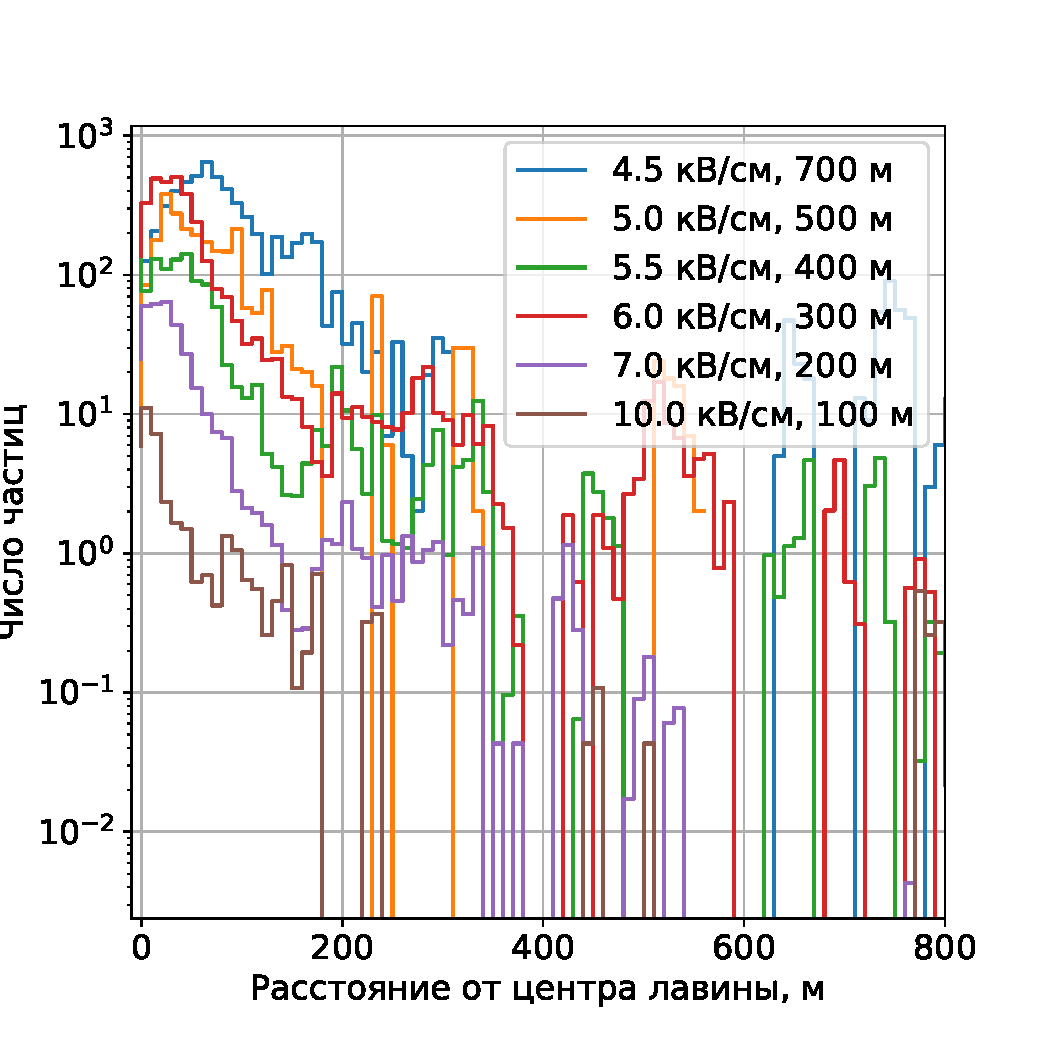
\includegraphics[width=\linewidth]{thunderstorm/rdfm/radial_positron.pdf}   \\ б)}
        \end{minipage}
        \caption{Радиальное распределение затравочных электронов рожденных за счет а) гамма обратной связи б) позитронной обратной связи.}
    \end{center}
    \label{fig:storm:radial_fb}
\end{figure}


Так важно учесть не только распределение в горизонтальном пространстве, но и по вертикали. Обычно в моделировании мы размещаем затравочную частицу в начале области с электрическим полем, однако новые затравочные частицы рождаемые за счет гамма или позитронной обратной связи имеют некоторое распределение по вертикали,  и поэтому для новой затравочной частицы длинна области с поле будет эффективно сокращаться по сравнению с длинной облака для первой затравочной частицы. Попробуем оценить как влияет это сокращение на работу механизмов обратной связи. Пусть расстояние от центра облака до его верхнего края равно $H$, именно в этой части рождаются новые затравочные частицы, разобьем это пространство на $N$ слоёв толщиной $\Delta h$, и подсчитаем с учетом вероятности разворота число $n(i)$ новых затравочных частиц на одну первичную частицу в $i$-том слое. Чтобы упростить расчеты и не учитывать влияние значения энергии и направления импульса частиц будем считать что все новые частицы могут порождать новые лавины также эффективно как первичная частица. Частицы расположенные в самом верхнем $N$-том слое считаются тождественными начальной частицы и если считать что на $j$-ой итерации в этом слое находится $k(N)^j$ частиц, то тогда на каждой итерации эти частицу будут создавать $n(i)*k(N)^j$ частиц в $i$-том слое. С частицами из следующих слоев сложнее, для частиц расположенных в $N-1$ слое с одной стороны расстояние на котором происходит развитие лавины уменьшилось, с другой над этими частица появилась область с полем: когда мы рассматриваем затравочную частицу инжектированную в самый верх облака, мы игнорируем частицы рожденные выше её, так как там находится область без поля, теперь же появилась дополнительная область где гамма-кванты и позитроны могут создавать затравочные частицы. В нашей оценке трудно точным образом учесть эти факторы, но поскольку они имеют разную направленность и могут компенсировать друг друга, давайте рассмотрим такую модель:  будем рассматривать частицы как будто они инжектированы в верную часть объема и производят соответствующим образом распределенные затравочные частицы, однако будет брать из этого распределения только ту часть которая, ложится на границы между выбранным слоем и серединой облака. Иначе говоря мы будет считать что если в некотором слое $l$ на $j$-ой итерации содержится $k(l)^j$ частиц, то они будут генерировать затравочные частицы только в слоях от первого до $l$-ого включительно, причем число сгенированных частиц в  $i$-том слое будет равно $k(l)^j * n(i+N-l)$. Теперь можно посчитать сколько частиц генерируется в слое за одну итерацию:
\begin{equation}
P(i)^{j} = \sum_{l=i}^{N} k(l)^j * n(i+N-l)
\end{equation}
Приведенный код на языке Python позволяет вычислить число частиц для заданной итерации:
\begin{lstlisting}[language=Python]
import numpy as np

def feedback(distrubution : np.ndarray, max_iteration: int) -> np.ndarray:
    distrubution = distrubution[::-1]
    for i in range(max_iteration):
        temp = np.zeros(distrubution.size)
        for indx, it in enumerate(distrubution):
            if indx == 0:
                temp = it*distrubution
            else:
                temp[indx:] += it*distrubution[:-indx]
        distrubution = temp
    return distrubution
\end{lstlisting}
Данная функция принимает в качестве аргумента \textit{distrubution} массив значений $n(i)$ для каждого слоя, а аргумент \textit{max\_iteration} задает итерацию для которой вычисляется конечное число частиц. На графике приведены количество частиц на разных итерация обратной связи для нескольких симуляций с разными значения электрического поля и длинны облака, величина $\Delta h$ во всех симуляциях взята равной 10 метрам. 

Рассмотрим результаты моделирования: в двух случаях мы видим гигантский рост частиц как и предсказывает Дуайер, однако в трех других случаях обратная связь затухает --- сказывается недостаток частиц в верхней частиц облака. Отсюда можно сделать несколько выводов: 
\begin{itemize}
    \item Полученных Дуаером условий может быть недостаточным для возникновения обратной связи, параметры определенные им в работе ~\cite{} могут быть не достаточны, и требуется увеличение электрического поля, однако при увеличении поля свыше 10 кВ/см мы попадем в область где уже становится возможным возникновения обычного электрического пробоя, и потому рассмотрение пробоя на убегающих электронов становится избыточным;
    \item Подтверждается тезис о том что увеличение длинны облака эффективнее чем усиление поля;
    \item Исходя из предыдущего пункта можно оспорить тезис Дуаера о том что механизмы обратной связи позволяют опровергнуть гипотезу о наличии скрытых внутриоблачным областей с сильным полем, как мы видим из моделирования как раз для такого случая (малый размер, сильное поле) механизмы обратной связи быстро затухают из-за смещения точки рождения затравочных частиц от верхнего края облака;
\end{itemize}

\begin{figure}[ph!]
    \begin{center}
        \begin{minipage}[h]{0.49\linewidth}
            \center{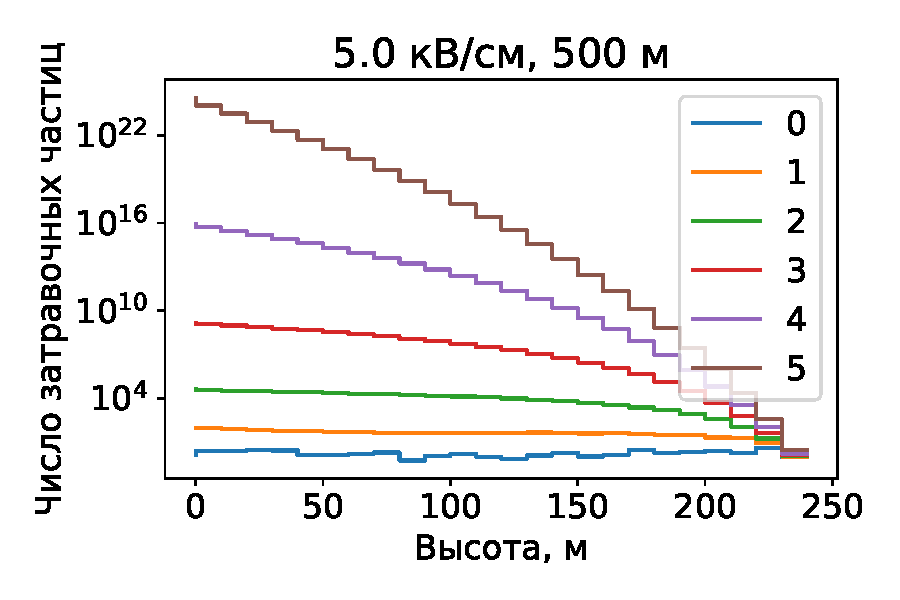
\includegraphics[width=\linewidth]{thunderstorm/rdfm/vertical_gamma_5_0.pdf} \\ а)}
        \end{minipage}
        \hfill
        \begin{minipage}[h]{0.49\linewidth}
            \center{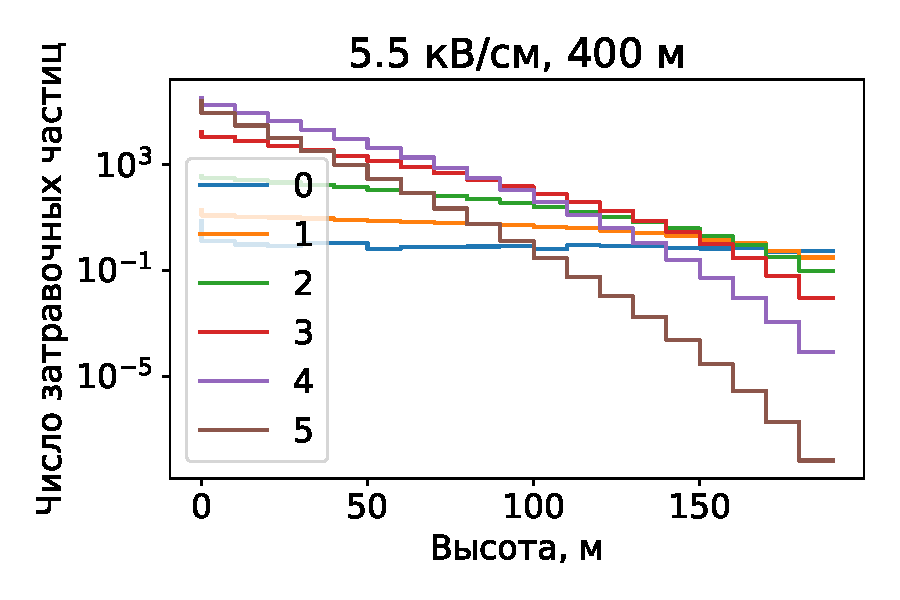
\includegraphics[width=\linewidth]{thunderstorm/rdfm/vertical_gamma_5_5.pdf} \\ б)}
        \end{minipage}
        \vfill
        \begin{minipage}[h]{0.49\linewidth}
            \center{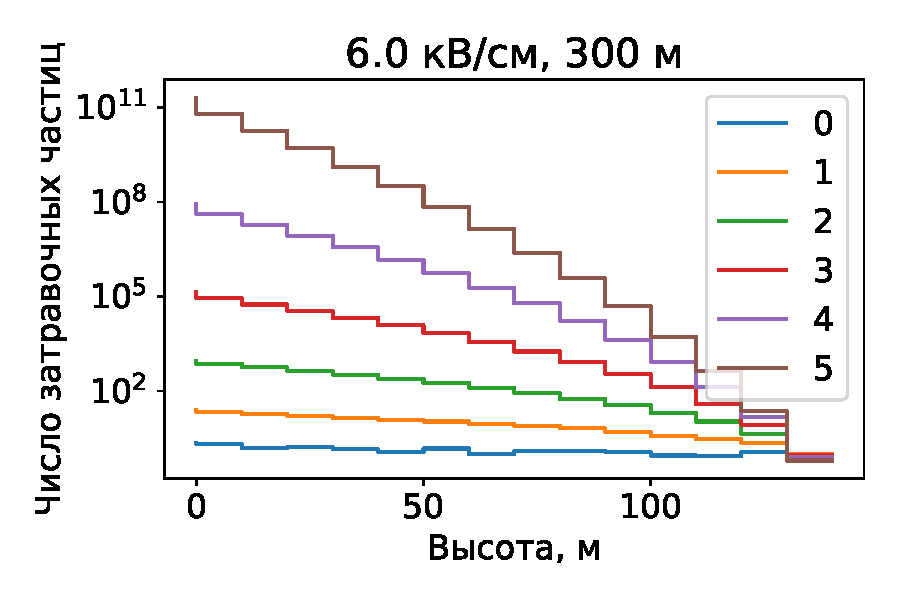
\includegraphics[width=\linewidth]{thunderstorm/rdfm/vertical_gamma_6_0.pdf} \\ в)}
        \end{minipage}
        \hfill
        \begin{minipage}[h]{0.49\linewidth}
            \center{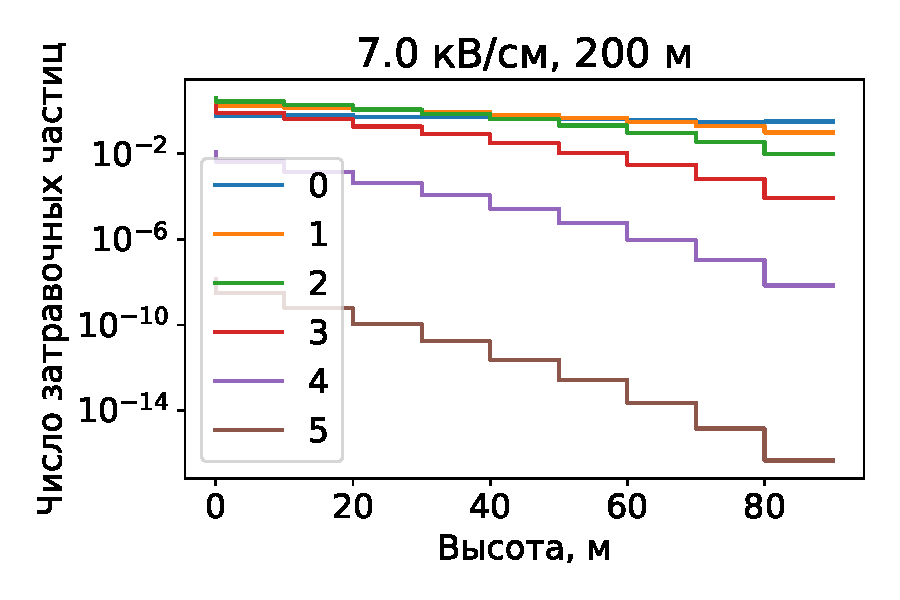
\includegraphics[width=\linewidth]{thunderstorm/rdfm/vertical_gamma_7_0.pdf} \\ г)}
        \end{minipage}
        \vfill
        \begin{minipage}[h]{0.49\linewidth}
            \center{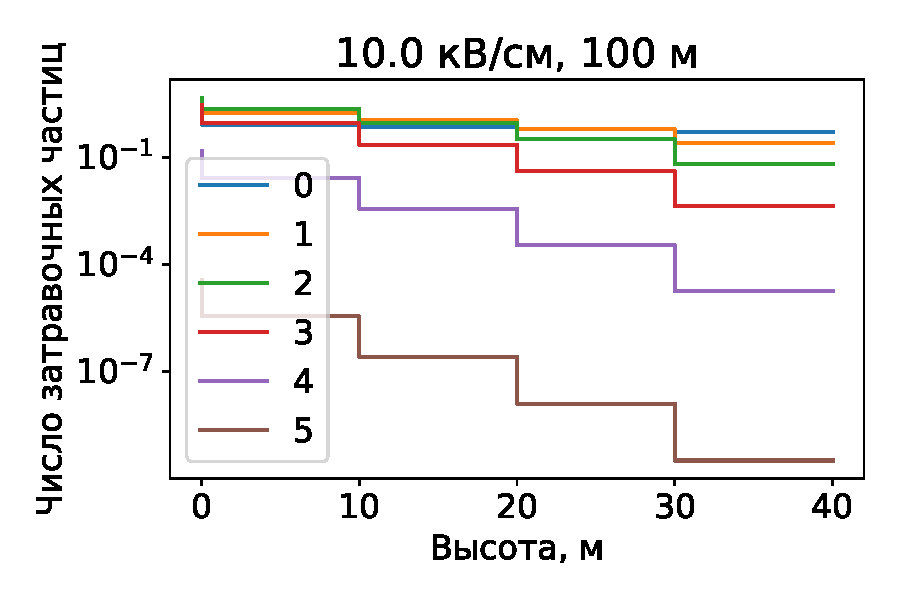
\includegraphics[width=\linewidth]{thunderstorm/rdfm/vertical_gamma_10_0.pdf} \\ д)}
        \end{minipage}
        \caption{Моделирование гамма обратной связи для различных облаков, на графиках приведено распределенное по высоте число частиц, на различных итерациях обратной связи, нулевая итерация соответствует частицам рожденным первичной затравочной частицей.}
    \end{center}
    \label{fig:storm:vertical_gamma}
\end{figure}
\begin{figure}[ph!]
    \begin{center}
        \begin{minipage}[h]{0.49\linewidth}
            \center{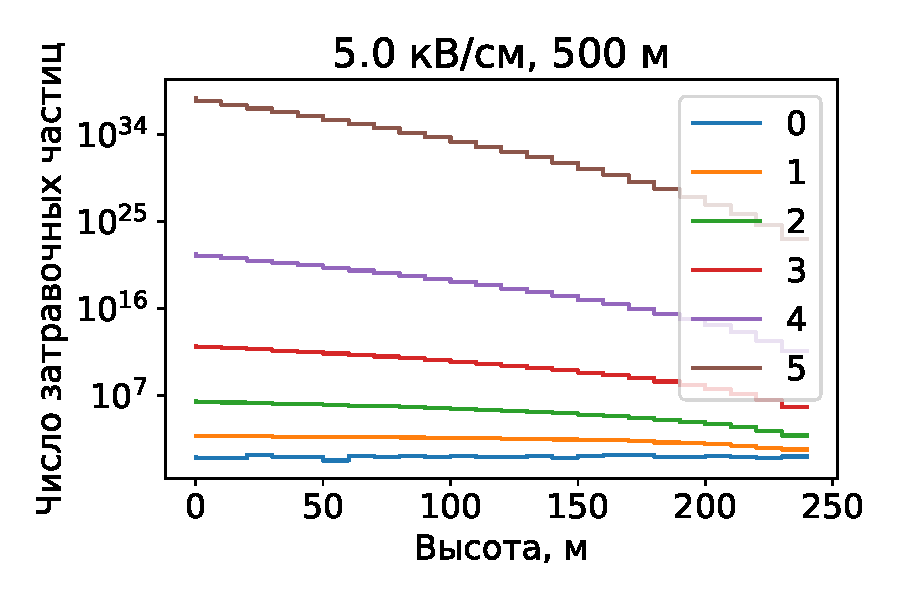
\includegraphics[width=\linewidth]{thunderstorm/rdfm/vertical_positron_5_0.pdf} \\ а)}
        \end{minipage}
        \hfill
        \begin{minipage}[h]{0.49\linewidth}
            \center{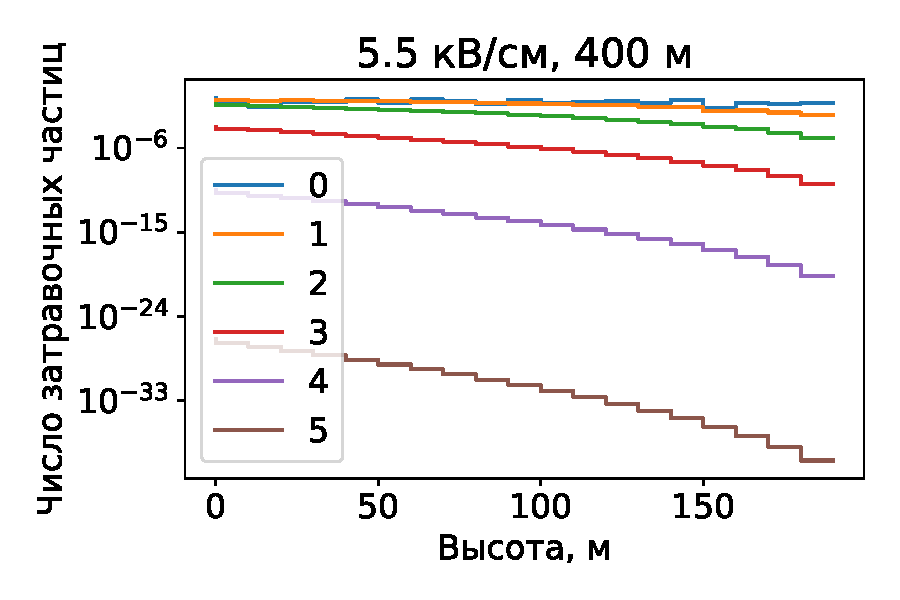
\includegraphics[width=\linewidth]{thunderstorm/rdfm/vertical_positron_5_5.pdf} \\ б)}
        \end{minipage}
        \vfill
        \begin{minipage}[h]{0.49\linewidth}
            \center{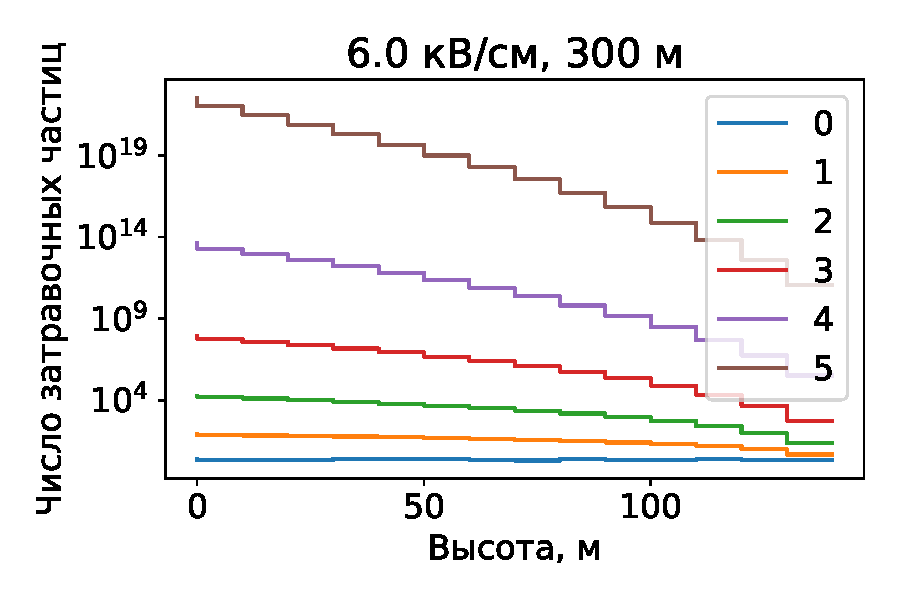
\includegraphics[width=\linewidth]{thunderstorm/rdfm/vertical_positron_6_0.pdf} \\ в)}
        \end{minipage}
        \hfill
        \begin{minipage}[h]{0.49\linewidth}
            \center{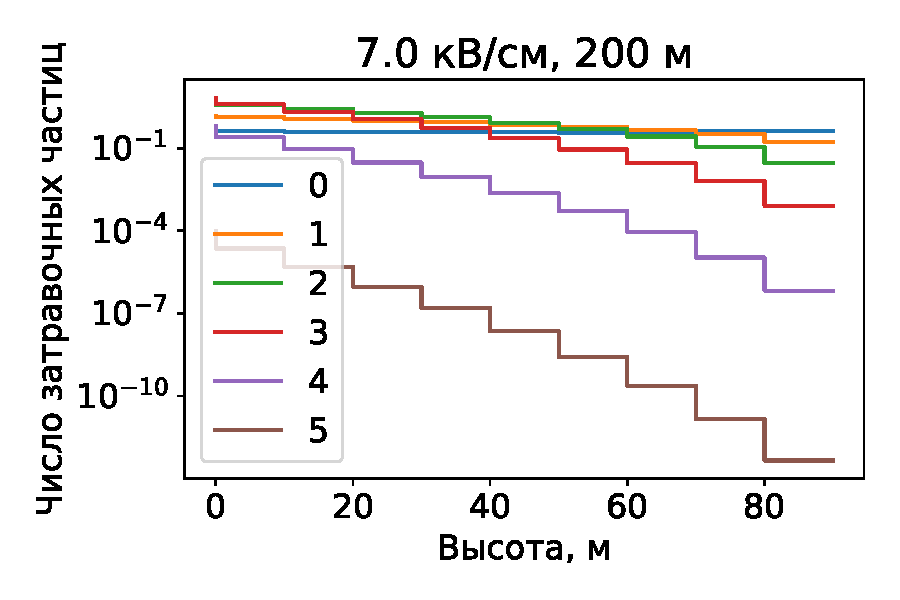
\includegraphics[width=\linewidth]{thunderstorm/rdfm/vertical_positron_7_0.pdf} \\ г)}
        \end{minipage}
        \vfill
        \begin{minipage}[h]{0.49\linewidth}
            \center{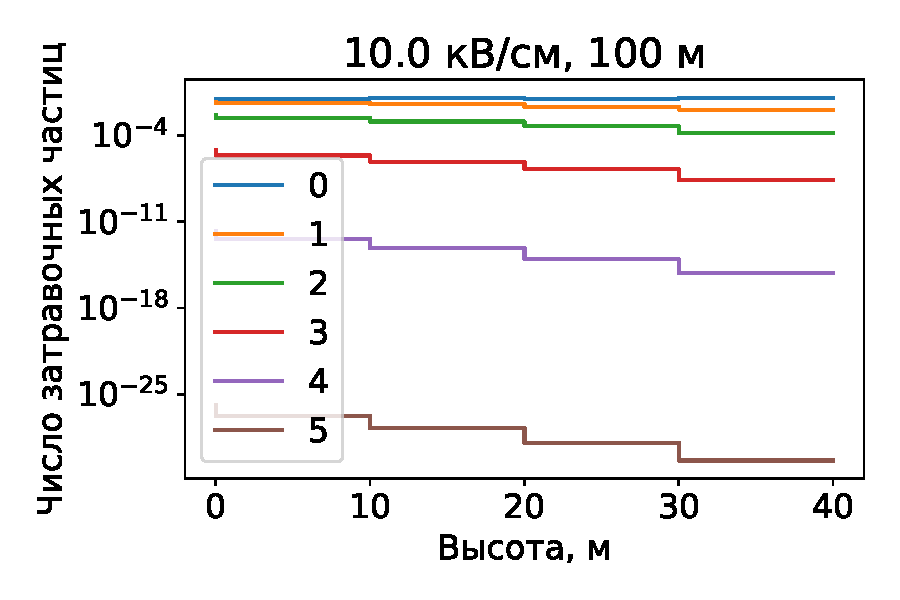
\includegraphics[width=\linewidth]{thunderstorm/rdfm/vertical_positron_10_0.pdf} \\ д)}
        \end{minipage}
        \caption{Моделирование позитронной обратной связи для различных облаков, на графиках приведено распределенное по высоте число частиц, на различных итерациях обратной связи, нулевая итерация соответствует частицам рожденным первичной затравочной частицей.}
    \end{center}
    \label{fig:storm:vertical_gamma}
\end{figure}

Пока мы следуя работе Дуайера проводили моделирование при нормальных условиях, однако как уже отмечалось не совсем корректно экстраполировать эти результаты на большие высоты. Поэтому в данной работе мы рассмотрим моделирование на больших высотах, соответствующее более реалистичным условиям, а именно возьмем плотность воздуха 0.5 кг/м$^3$, что примерно соответствует высоте в 8 километров, реалистичные значения электрического поля в атмосфере не превышают 2.25 кВ/см, поэтому мы возьмем для моделирования диапазон значение от 1 до 2.25 кВ/см, так же мы наложим ограничения на размер облака, оно будет представлять собой куб со стороной 400 метров. На основе данного моделирования рассчитан коэффициенты гамма и позитронной обратной связи (при подсчете затравочных электронов, также как и раннее учитывалась возможность разворота, смотри рисунок~\ref{fig:storm:ayss2018}а), зависимость которых от поля отображена на рисунке~\ref{fig:storm:ayss2018}б. Как мы видим даже в самом оптимистичном сценарии вклад обратной связи в рост числа электронов в лавине не превышает 10~\%. Методика и результаты этого моделирования представлены в работе~\cite{antidwyer} 

\begin{figure}[t]
    \begin{center}
        \begin{minipage}[h]{0.49\linewidth}
            \center{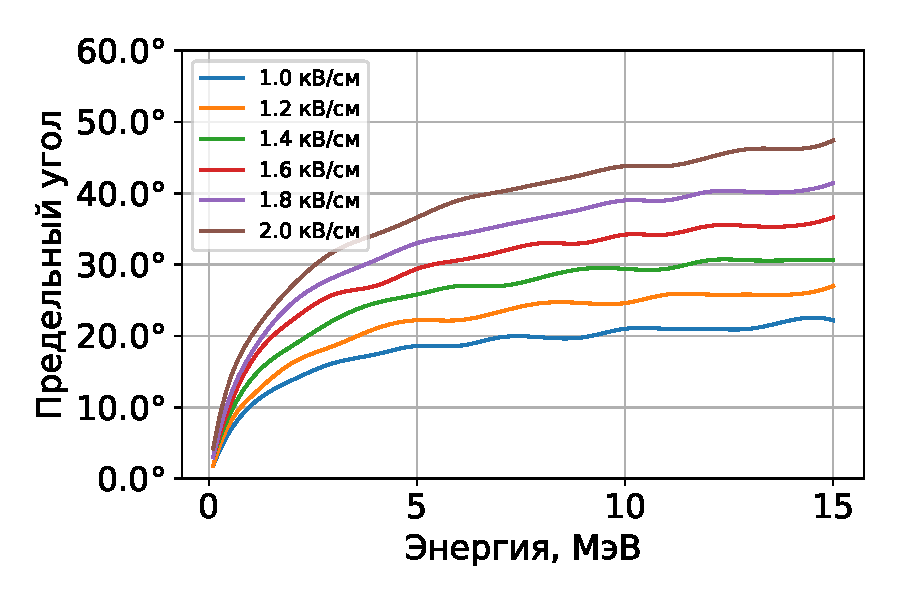
\includegraphics[width=\linewidth]{thunderstorm/ayss_2018_rev.pdf} \\ а)}
        \end{minipage}
        \hfill
        \begin{minipage}[h]{0.49\linewidth}
            \center{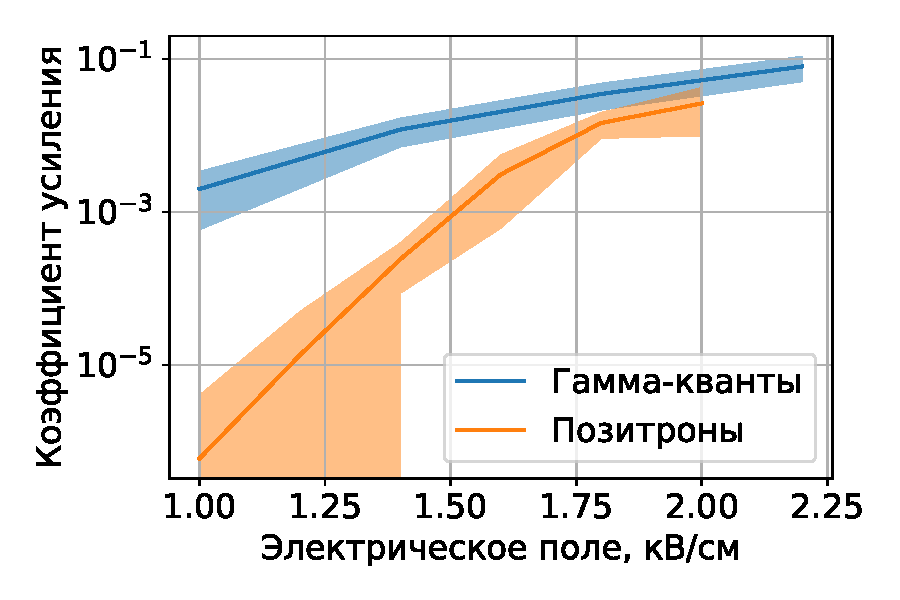
\includegraphics[width=\linewidth]{thunderstorm/ayss_2018_fb.pdf}   \\ б)}
        \end{minipage}
        \caption{а) Предельный угол между направление движения электрона и электрическим полем при котором происходит разворот электрона. б)Коэффициент гамма и позитронной обратной связи для следующих параметров: энергия затравочного электрона --- 3 МэВ, размер области с полем --- 400 метров, плотность воздуха --- 0.5 кг/м$^3$ ($\sim 0.5$ атм).}
    \end{center}
    \label{fig:storm:ayss2018}
\end{figure}
Подводя итоги этого раздела можно сказать что не смотря на то что по результатам моделирования проведенного в разделе~\ref{sec:thunderstorm/rrea}, учет гамма-квантов и позитронов необходим, достоверно утверждать что они могут запускать механизм приводящие к взрывному числа частиц нельзя, что подтверждается рядом экспериментальных наблюдений (TODO(ссылка на Чилингаряна)) 